\chapter{The extended ray mapping}
\label{chap:raymapping2}
In Chapter \ref{chap:raymapping1} we introduced an inverse method based on a ray mapping reconstruction in PS.
The goal was to calculate the intensity distribution at the target of optical systems. 
The idea was to construct a map from the target \point{T} to the source \point{S} using the PS of all the optical lines which are divided into several regions.  
The method developed in the previous chapter requires that the boundaries of the regions of every PS can be determined exactly. This is possible for systems formed by straight line segments.
The results found show that the procedure allows tracing the only rays located
 on the boundaries of the regions with positive luminance. From these rays, the output intensity is calculated. Since the boundaries in PS are computed analytically, the output intensity is the \textit{exact} intensity. \\ \indent
In this chapter we extend the method to systems formed by curved lines. In this case, the boundaries of the regions that form the PS cannot be determined exactly.
Because of this, we need to use a numerical procedure. In particular, we develop a method that employs only the PS of the target of the system. 
The boundaries are detected applying sequentially a bisection procedure in target PS and the inverse ray tracing procedure.\\ \indent
The details are explained in the next section. In this chapter we test the method for two optical systems: the TIR-collimator and a parabolic reflector. The results are presented in Section \ref{sec:TIR} and \ref{sec:PR}, respectively.
\section{Explanation of the method}
The purpose of this section is to present the generalized inverse ray mapping method valid for systems formed by curved lines. 
Given a partition $-1 = \variabile{p}^0<\variabile{p}^1<\cdots<\variabile{p}^{\nbin}$ of the interval $[-1,1]$ with $\nbin$ the number of rays in the partitioning, the intensity in target PS is given by Equation (\ref{eta2}) for every $\dir{}{}\in P$.
Therefore, the problem reduces to calculate the coordinates 
$\variabile{q}^{\textrm{\,min}}(\Pi, \variabile{p})$ and $\variabile{q}^{\textrm{\,max}}(\Pi, \variabile{p})$ of the rays on $\partial$\set{R}{}{}$(\Pi)$ for every path $\Pi$.\\ \indent 
Using the same idea of the analytic ray mapping, for a given direction $\variabile{p}$, the procedure starts considering $I(p)=0$ and the end points $(\variabile{q}^{\,\textrm{a}}, \variabile{p})= (-\variabile{b}, \variabile{p})$ and $(\variabile{q}^{\,\textrm{b}}, \variabile{p}) = (\variabile{b}, \variabile{p})$ of \set{T}{}{} along direction $\variabile{p}$. We indicate with $\vect{r}_{\textrm{a}}$ and $\vect{r}_{\textrm{b}}$ the corresponding rays of these two points. Now, since the boundaries of the PS are unknown\footnote{More precisely we know only the boundaries of the region of the target PS and we cannot calculate exactly the boundaries of the other phase space.}, to understand from which line $\vect{r}_{\textrm{a}}$ and $\vect{r}_{\textrm{b}}$ are illuminated we apply the inverse ray tracing. We denote with $\nline$ the index of the target (line $\nline$) and with $\lineaj\in\{1,\cdots, \nline-1\}$ and $\lineak\in\{1,\cdots, \nline-1\}$ the lines from which $\vect{r}_{\textrm{a}}$ and $\vect{r}_{\textrm{b}}$ are emitted, respectively. $\Pi_\textrm{a} = (\lineaj, \nline)$ and $\Pi_\textrm{b} = (\lineak,\nline)$ are the paths followed by the two rays $\vect{r}_{\textrm{a}}$ and $\vect{r}_{\textrm{b}}$, respectively. At this stage we know whether the two rays are emitted or not by the same line. \\ \indent 
If $\lineaj= \lineak$, then $\vect{r}_{\textrm{a}}$ and $\vect{r}_{\textrm{b}}$ are hit the same line before reaching the target. 
In case $\lineaj = 1$ a possible path from the source to the target is found and the intensity is updated according to:
\begin{equation}
I(p) = I(p)+\variabile{q}^{\textrm{max}}(\Pi_\textrm{a}, \variabile{p})-\variabile{q}^{\textrm{min}}(\Pi_\textrm{a}, \variabile{p}),
\end{equation}
where $\variabile{q}^{\textrm{min}} = \min\{\variabile{q}^{\textrm{a}}, \variabile{q}^{\textrm{b}}\}$ and $\variabile{q}^{\textrm{max}} = \max\{\variabile{q}^{\textrm{a}}, \variabile{q}^{\textrm{b}}\}$. In case $\lineaj\neq1$ the two rays $\vect{r}_{\textrm{a}}$ and $\vect{r}_{\textrm{b}}$ are traced back again using the inverse ray tracing with the corresponding coordinates of each ray on line $\lineaj$.
\\ \indent If $\lineaj\neq \lineak$ the rays $\vect{r}_\textrm{a}$ and $\vect{r}_\textrm{b}$ are emitted by two-different lines, hence $\Pi_{\textrm{a}}\neq \Pi_{\textrm{b}}$ and belong to different regions \set{R}{}{}$(\Pi_{\textrm{a}})$ and \set{R}{}{}$(\Pi_{\textrm{b}})$ in \set{T}{}{}. To determine the ray on the boundary $\partial$\set{R}{}{}$(\Pi_{\textrm{a}})$, the bisection method is applied to the interval $[\variabile{q}^{\,\textrm{a}}(\Pi_{\textrm{a}}, \variabile{p}), \variabile{q}^{\,\textrm{b}}(\Pi_{\textrm{b}}, \variabile{p})]$ in target \set{}{}{} along direction $\variabile{p}$. Thus, this interval is halves until the coordinates in target PS of the ray that follows the same path $\Pi_{\textrm{a}}$ of ray $\vect{r}_{\textrm{a}}$ are found. \\ \indent Bisection procedure continues until the length of the segment considered becomes smaller than a fixed tolerance. 
Giving as input the coordinates $\variabile{q}^{\,\textrm{a}}(\Pi_{\textrm{a}}, \variabile{p})$ and $\variabile{q}^{\,\textrm{b}}(\Pi_{\textrm{b}}, \variabile{p})$ of $\vect{r}_{\textrm{a}}$ and $\vect{r}_{\textrm{b}}$, the path $\Pi_\textrm{a}$ and the tolerance $\textrm{tol}= 10^{-12}$, the bisection method is implemented as in Algorithm \ref{alg:bisection}.
\begin{algorithm}
\caption{Bisection}\label{alg:bisection}
Initialize $\textrm{step} = 0$
\begin{algorithmic}[1]
\While {$|\variabile{q}^{\,\textrm{a}}-\variabile{q}^{\,\textrm{b}}|>\textrm{tol}$}
\State $\Pi_{\textrm{m}}\gets \nline,$
\State $\variabile{q}^{\,\textrm{m}}\gets \frac{\variabile{q}^{\,\textrm{a}}+\variabile{q}^{\,\textrm{b}}}{2},$ 
\State $\variabile{p}^{\,\textrm{m}}\gets\variabile{p},$
\State $\vect{r}_{\textrm{m}}\gets \variabile{q}^{\,\textrm{m}}+s \variabile{p}^{\,\textrm{m}}$ with $s>0$ the arc-length,
\While {$\textrm{step}<\mbox{length}(\Pi_\textrm{a})-1$}
\State Apply the inverse of ray tracing to the corresponding coordinates of $\vect{r}_{\textrm{m}}$ on line $\lineaj$,
\State Find the line $\lineak$ that the ray $\vect{r}_{\textrm{m}}$ hits.
\State $\Pi_{\textrm{m}}\gets (\lineak,\Pi_{\textrm{m}})$.
\If {$\lineak=1$ or $\lineak=\nline$}
\State $\textrm{step} = \mbox{length}(\Pi_\textrm{a})$ \Comment If the source or the target are reached \\  \Comment then exit from the while loop.
\Else \State $\textrm{step}\gets\textrm{step}+1$ 
\EndIf
\EndWhile
\If {$\Pi_\textrm{a} = \Pi_\textrm{m}$}
\State $(\variabile{q}^{\,\textrm{a}}, \variabile{p}^{\,\textrm{a}})\gets (\variabile{q}^{\,\textrm{m}}, \variabile{p})$
\State $\vect{r}_{\textrm{a}}\gets \vect{r}_{\textrm{m}}$
\Else 
\State $(\variabile{q}^{\,\textrm{b}}, \variabile{p}^{\,\textrm{b}})\gets (\variabile{q}^{\,\textrm{m}}, \variabile{p}^{\,\textrm{m}})$
\State $\vect{r}_{\textrm{b}}\gets \vect{r}_{\textrm{m}}$
\State $\Pi_\textrm{b}\gets \Pi_{\textrm{m}}$
\EndIf
\EndWhile
\State $(\variabile{q}^{\,\textrm{c}}, \variabile{p}^{\,\textrm{c}})\gets (\variabile{q}^{\,\textrm{a}}, \variabile{p}^{\,\textrm{a}}), \Pi_\textrm{c}\gets \Pi_{\textrm{a}}.$
\State $(\variabile{q}^{\,\textrm{d}}, \variabile{p}^{\,\textrm{d}})\gets (\variabile{q}^{\,\textrm{b}}, \variabile{p}^{\,\textrm{b}}), \Pi_\textrm{d}\gets \Pi_{\textrm{b}}.$
\State \Return $(\variabile{q}^{\,\textrm{c}}, \variabile{p}^{\,\textrm{c}})$, $(\variabile{q}^{\,\textrm{d}}, \variabile{p}^{\,\textrm{d}})$, $\Pi_{\textrm{c}}$ and $\Pi_{\textrm{d}}$.
\end{algorithmic}
\end{algorithm}
\\ \indent Once bisection stops, two points with coordinates $(\variabile{q}^{\,\textrm{c}}, \variabile{p})$ and $(\variabile{q}^{\,\textrm{d}}, \variabile{p})$ in \set{T}{}{} are found. The corresponding rays $\vect{r}_{\textrm{c}}$ and $\vect{r}_{\textrm{d}}$ follow path $\Pi_{\textrm{c}}=\Pi_{\textrm{a}}$ and $\Pi_{\textrm{d}}\neq\Pi_{\textrm{a}}$, respectively. 
All the rays with target coordinates $(\variabile{q}, \variabile{p})$ and $\variabile{q}^{\,\textrm{a}}\leq\variabile{q}\leq\variabile{q}^{\,\textrm{c}}$ follow path $\Pi = \Pi_{\textrm{a}}$, while the rays with target coordinates $(\variabile{q}, \variabile{p})$ with $\variabile{q}^{\,\textrm{d}}\leq\variabile{q}\leq\variabile{q}^{\,\textrm{b}}$ follow another path $\Pi \neq \Pi_{\textrm{a}}.$ 
% To clarify the concept, in Figure \ref{fig:bisec} we show the target PS of an optical system where Algorithm \ref{alg:bisection} is  applied to the interval $[]$ along direction $\variabile{p}=0$. The paths followed by the corresponding rays are different $$. The bisection procedure is applied in order to find the coordinated of the ray that follow path . The coordinates $$ and $$ of two points at the target PS and the paths $\Pi_{\textrm{c}}$ and $\Pi_{\textrm{d}}$ that the corresponding rays follow are found. $\Pi_{\textrm{c}}$ and 
%
\\ \indent Now, in order to determine the boundaries of \textrm{all} the patches formed by the rays that are illuminated by the source, the procedure previously applied to the interval 
$[\variabile{q}^{\textrm{a}}(\variabile{p}), \variabile{q}^{\textrm{b}}(\variabile{p})]$ needs to be applied to $[\variabile{q}^{\textrm{a}}(\variabile{p}),\variabile{q}^{\textrm{c}}(\variabile{p})]$ until the source is reached, i.e. until $\lineaj=1$. When $\lineaj=1$, the source is reached by the rays traced back from the target. This means that a possible path $\Pi$ is found and the position coordinates $\variabile{q}^{\textrm{\,min}}(\Pi, \variabile{p})$ and $\variabile{q}^{\textrm{\,max}}(\Pi, \variabile{p})$ on \set{T}{}{} of the rays located at the boundaries $\partial$\set{R}{}{}$(\Pi)$ of the rays that follow that path are determined. \\ \indent 
Finally, to detect all the possible paths that can occur along direction $\variabile{p}$ the procedure explained above is applied also to the segment $[\variabile{q}^{\textrm{d}}(\variabile{p}), \variabile{\textrm{b}}]$ along direction $\variabile{p}$. 
The main steps of the method are outlined in the following.
\begin{enumerate}
\item Given a direction \variabile{p}, consider the end points $(\variabile{q}^{\,\textrm{a}}, \variabile{p})$ and $(\variabile{q}^{\,\textrm{b}}, \variabile{p})$ of the target PS \set{T}{}{}.
\item \label{ray trace} Trace back the rays $\vect{r}_{\textrm{a}}$ and $\vect{r}_\textrm{b}$ corresponding to the coordinates  $(\variabile{q}^{\,\textrm{a}}, \variabile{p})$ and $ (\variabile{q}^{\,\textrm{b}}, \variabile{p})$ using the inverse ray tracing procedure,
\item Determine indices $\lineaj$ and $\lineak$ of the lines that  $\vect{r}_{\textrm{a}}$ and $\vect{r}_{\textrm{b}}$  hit, respectively.\\
\item Update the paths $\Pi_\textrm{a}$ and $\Pi_\textrm{b}$ of rays $\vect{r}_\textrm{a}$ and $\vect{r}_\textrm{b}$, respectively.  $\Pi_\textrm{a} = (\lineaj, \Pi_{\textrm{a}})$ and $\Pi_\textrm{b} = (\lineak, \Pi_\textrm{b}),$
\item If $\lineaj=\lineak \neq 1$ 
\begin{itemize}
\item Restart the procedure from point $\ref{ray trace}$ considering the coordinates of rays $\vect{r}_{\textrm{a}}$ and $\vect{r}_{\textrm{b}}$ on line $\lineaj$ 
\end{itemize}
\item If $\lineaj=\lineak= 1$ 
\begin{itemize}
\item A relevant path $\Pi_{\textrm{a}}$ is found. 
\item Determine 
\begin{equation*}
\begin{aligned}
\variabile{q}^{\textrm{min}}(\Pi_{\textrm{a}}, \variabile{p})&=\min\{\variabile{q}^{\textrm{a}}(\Pi_{\textrm{a}}, \variabile{p}), \variabile{q}^{\textrm{c}}(\Pi_{\textrm{a}}, \variabile{p})\}\\ 
\variabile{q}^{\textrm{max}}(\Pi_{\textrm{a}}, \variabile{p})&=\max\{\variabile{q}^{\textrm{a}}(\Pi_{\textrm{a}}, \variabile{p}), \variabile{q}^{\textrm{c}}(\Pi_{\textrm{a}}, \variabile{p})\},
\end{aligned}
\end{equation*}
\item Update the intensity $$I(\variabile{p}) = I(p)+\variabile{q}^{\textrm{max}}(\Pi_{\textrm{a}}, \variabile{p})-\variabile{q}^{\textrm{min}}(\Pi_{\textrm{a}}, \variabile{p})$$
\end{itemize}
\item If $\lineaj\neq\lineak$ 
\begin{itemize}
\item Apply the bisection method to the interval $[\variabile{q}^{\textrm{a}}, \variabile{q}^{\textrm{b}}]$ along direction $\variabile{p}$.
\item Find the points with coordinates $(\variabile{q}^{\,\textrm{c}}, \variabile{p})$ and $(\variabile{q}^{\,\textrm{d}}, \variabile{p})$ in target PS \set{T}{}{} where $|\variabile{q}^{\,\textrm{c}}-\variabile{q}^{\,\textrm{d}}|<\textrm{tol}$ and $\textrm{tol}=10^{-12}$ is the tolerance in the bisection procedure. 
\item Consider the segment $[\variabile{q}^{\textrm{a}}(\variabile{p}),\variabile{q}^{\textrm{c}}(\variabile{p})]$,
\item Restart from $\ref{ray trace}$ considering the end points of $[\variabile{q}^{\textrm{a}}(\variabile{p}),\variabile{q}^{\textrm{c}}(\variabile{p})]$,
\end{itemize}
\item Restart from $\ref{ray trace}$ with coordinates $\variabile{q}^{\textrm{d}}$ and $\variabile{q}^{\textrm{b}}$,
\item If $\lineaj=\lineak= \nline$ stop the procedure (the rays reach the target again).
\end{enumerate}
The method is developed using the recursive Algorithm \ref{alg:recursiveraymapping}.
% Insert algorithm
\begin{algorithm}
\caption{Recursive function for the extended ray mapping}\label{alg:recursiveraymapping}
Initialize $\lineai = \nline$, $\variabile{q}^{\,\textrm{a}}= \variabile{q}^{\,\textrm{a}}_{\lineai}=-\variabile{b}$, $\variabile{q}^{\,\textrm{b}}= \variabile{q}^{\,\textrm{b}}_{\lineai}=\variabile{b}$, $\dir{}{}=\variabile{p}^{\textrm{a}}_\lineai=\variabile{p}^{\textrm{b}}_\lineai=\textrm{const}$, $\Pi_{\textrm{a}}=({\nline})$.
\begin{algorithmic}[1]
\Procedure {Intensity computation}{$\variabile{q}^{\,\textrm{a}}$,  $\variabile{q}^{\,\textrm{b}}$, $\variabile{q}^{\,\textrm{a}}_{\lineai},$  $\variabile{q}^{\,\textrm{b}}_{\lineai},$ $\dir{}{}$, $\variabile{p}^{\textrm{a}}_{\lineai}$, $\variabile{p}^{\textrm{b}}_{\lineai}$, $\Pi_{\textrm{a}}$, $\lineai$}
\State Apply the inverse ray tracing to the coordinates $(\variabile{q}^{\,\textrm{a}}_{\lineai},\variabile{p}^{\textrm{a}}_{\lineai})$ and $(\variabile{q}^{\,\textrm{b}}_{\lineai},\variabile{p}^{\textrm{b}}_{\lineai})$ on $\lineai$ of the rays $\vect{r}_{\textrm{a}}$ and $\vect{r}_{\textrm{b}}$.
\State Find the lines $\lineaj$ and $\lineak$ from which $\vect{r}_{\textrm{a}}$ and $\vect{r}_{\textrm{b}}$ are emitted, respectively.
\State Update path $\Pi_{\textrm{a}}\gets(\lineaj, \Pi_{\textrm{a}})$
\State Calculate the coordinates $(\variabile{q}^{\,\textrm{a}}_{\lineaj},\variabile{p}^{\textrm{a}}_{\lineaj})$ and $(\variabile{q}^{\,\textrm{b}}_{\lineaj}, \variabile{p}^{\textrm{b}}_{\lineaj})$ of $\vect{r}_{\textrm{a}}$ and $\vect{r}_{\textrm{b}}$ on line $\lineaj$
\If {$\lineaj = \lineak$}
\State Apply the inverse ray tracing to the coordinates $(\variabile{q}^{\,\textrm{a}}_{\lineaj},\variabile{p}^{\textrm{a}}_{\lineaj})$ and $(\variabile{q}^{\,\textrm{b}}_{\lineaj}, \variabile{p}^{\textrm{b}}_{\lineaj})$ on $\lineaj$ of the rays $\vect{r}_{\textrm{a}}$ and $\vect{r}_{\textrm{b}}$,
\If{$\lineaj\neq1$}
\State\Return{\Call{Intensity computation}{$\variabile{q}^{\,\textrm{a}},$  $\variabile{q}^{\,\textrm{b}},$ $\variabile{q}^{\,\textrm{a}}_{\lineaj},$ $\variabile{q}^{\,\textrm{b}}_{\lineaj},$ $\dir{}{}$, $\variabile{p}^{\textrm{a}}_{\lineaj}$, $\variabile{p}^{\textrm{b}}_{\lineaj}$, $\Pi_{\textrm{a}}$, $\lineaj$}}
\Else 
$I(\dir{}{}) = I(\dir{}{})+\variabile{q}^{\textrm{max}}(\Pi_{\textrm{a}}, \dir{}{})
-\variabile{q}^{\textrm{min}}(\Pi_{\textrm{a}}, \dir{}{}),$
\EndIf
\Else 
\State Apply bisection to the segment $[\variabile{q}^{\,\textrm{a}}(\Pi_\textrm{a}, \dir{}{}), \variabile{q}^{\,\textrm{b}}(\Pi_\textrm{b}, \dir{}{})]$
\State Find the target coordinates $(\variabile{q}^{\,\textrm{c}},\variabile{p})$ and $(\variabile{q}^{\,\textrm{d}},\variabile{p})$ of the rays $\vect{r}_{\textrm{c}}$ and $\vect{r}_{\textrm{d}}$, 
\If {$\lineaj\neq \nline$}
\State\Return{\Call{Intensity computation}{$\variabile{q}^{\,\textrm{a}},$  $\variabile{q}^{\,\textrm{c}},$ $\variabile{q}^{\,\textrm{a}}_{\lineaj},$ $\variabile{q}^{\,\textrm{c}}_{\lineaj},$ $\dir{}{}$, $\variabile{p}^{\textrm{a}}_{\lineaj}$, $\variabile{p}^{\textrm{b}}_{\lineaj}$, $\Pi_{\textrm{a}}$, $\lineaj$}}
\EndIf 
\State\Return{\Call{Intensity computation}{$\variabile{q}^{\,\textrm{c}},$  $\variabile{q}^{\,\textrm{d}},$ $\variabile{q}^{\,\textrm{c}}_{\lineaj},$ $\variabile{q}^{\,\textrm{d}}_{\lineaj},$ $\dir{}{}$, $\variabile{p}^{\textrm{a}}_{\lineaj}$, $\variabile{p}^{\textrm{b}}_{\lineaj}$, $\Pi_{\textrm{a}}$, $\lineaj$}}
\EndIf
\EndProcedure
\end{algorithmic}
\end{algorithm}
The explained procedure is able to determine all the possible paths that the rays can follow during their propagation from \set{S}{}{} to \set{T}{}{}. Also, the rays located exactly on the boundaries of the regions with positive luminance on target PS \set{T}{}{} are found.\\ \indent
Next, the method is applied to two example of optical systems formed by curved lines. In the next section we show the results for the TIR-collimator.
\section{Results for the TIR-collimator}\label{sec:TIR}
% Introduction 
In this section we apply the extended inverse ray mapping to the TIR-collimator presented in Chapter \ref{chap:boundaries_alpha} and depicted in Figure \ref{fig:analyticlens}. The target PS of this system is the rectangular \set{T}{}{}$= [-\variabile{b}, \variabile{b}]\times[-1,1]$ with $\variabile{b}=9.7$. The aim is to detect all the possible path $\Pi$ and the rays located on the boundaries $\partial$\set{R}{}{}$(\Pi)$ of the corresponding regions in target PS. 
\\ \indent In Chapter \ref{chap:boundaries_alpha} five different paths are found for the the TIR-collimator, and the boundaries of the corresponding regions in target PS \set{T}{}{} are in general difficult to approximate. Furthermore, along the same direction $\dir{}{}$ more than two points can be located on the boundary $\partial$\set{R}{}{}$(\Pi)$ of the region \set{R}{}{}$(\Pi)$ corresponding to a certain path $\Pi$. To determine properly all the boundaries 
$\partial$\set{R}{}{}$(\Pi)$, we need to divide the interval $[-\variabile{b}, \variabile{b}]$ in 
\set{T}{}{} into intervals of the same length (bins). Hence, we consider a partitioning 
$Q = -\variabile{b}=\variabile{q}^{0}<\variabile{q}^{1}<\cdots<\variabile{q}^{\textrm{Ni}}=\variabile{b}$ of $[-\variabile{b}, \variabile{b}]$ where $\textrm{Ni}$ is the total number of bins along the $\variabile{q}$-axis.
For each direction $\dir{}{}\in [-1,1]$ the procedure explained in Section \ref{chap:raymapping2} is repeated for every sub-interval $[\variabile{q}^{\textrm{k}}(\dir{}{}), \variabile{q}^{\textrm{k}+1}(\dir{}{})]\subset [\variabile{q}^{\textrm{a}}(\dir{}{}), \variabile{q}^{\textrm{b}}(\dir{}{})]$ with $\textrm{k}=0, \cdots, \textrm{Ni}-1$ and $\variabile{q}^{\textrm{a}}(\dir{}{}) = -\variabile{b}$ and $\variabile{q}^{\textrm{b}}(\dir{}{}) = \variabile{b}$.\\ \indent
To establish in how many \textrm{Ni} bins we need to divide the target, we exploit \'{e}tendue conservation. The same idea applied to determine the value of $\alpha$ for $\alpha$-shapes methods or to provide a stopping criterion for the triangulation refinement is used here, see Chapters \ref{} and \ref{}.
\begin{figure}[h]
  \begin{center}
  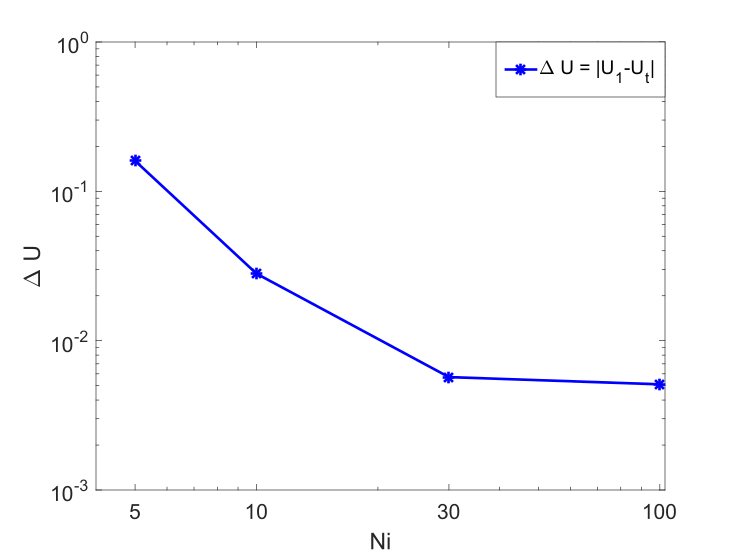
\includegraphics[width=0.7\textwidth]{etendue_raymapping_tir}
  \end{center}
  \caption{\textbf{Rays distribution at target PS of the TIR-collimator.}
 The $\variabile{q}$-axis is divided into $\textrm{Ni}=30$ bins, the $\variabile{p}$-axis is divided into $\nbin = 100$ bins. Using the ray mapping method only few rays are traced from the target to the source (red dots). Because of numerical error, few rays outside the region with positive luminance are found (Rays rimmed in red).}
\label{fig:boundaries_TIR_ray_mapping}
 \end{figure}
As an example, in Figure \ref{fig:boundaries_TIR_ray_mapping} we show the distribution of the rays traced using the inverse ray mapping method with $\textrm{Ni}=30$ and $\nbin = 100.$ 
\begin{figure}[h]
  \begin{center}
  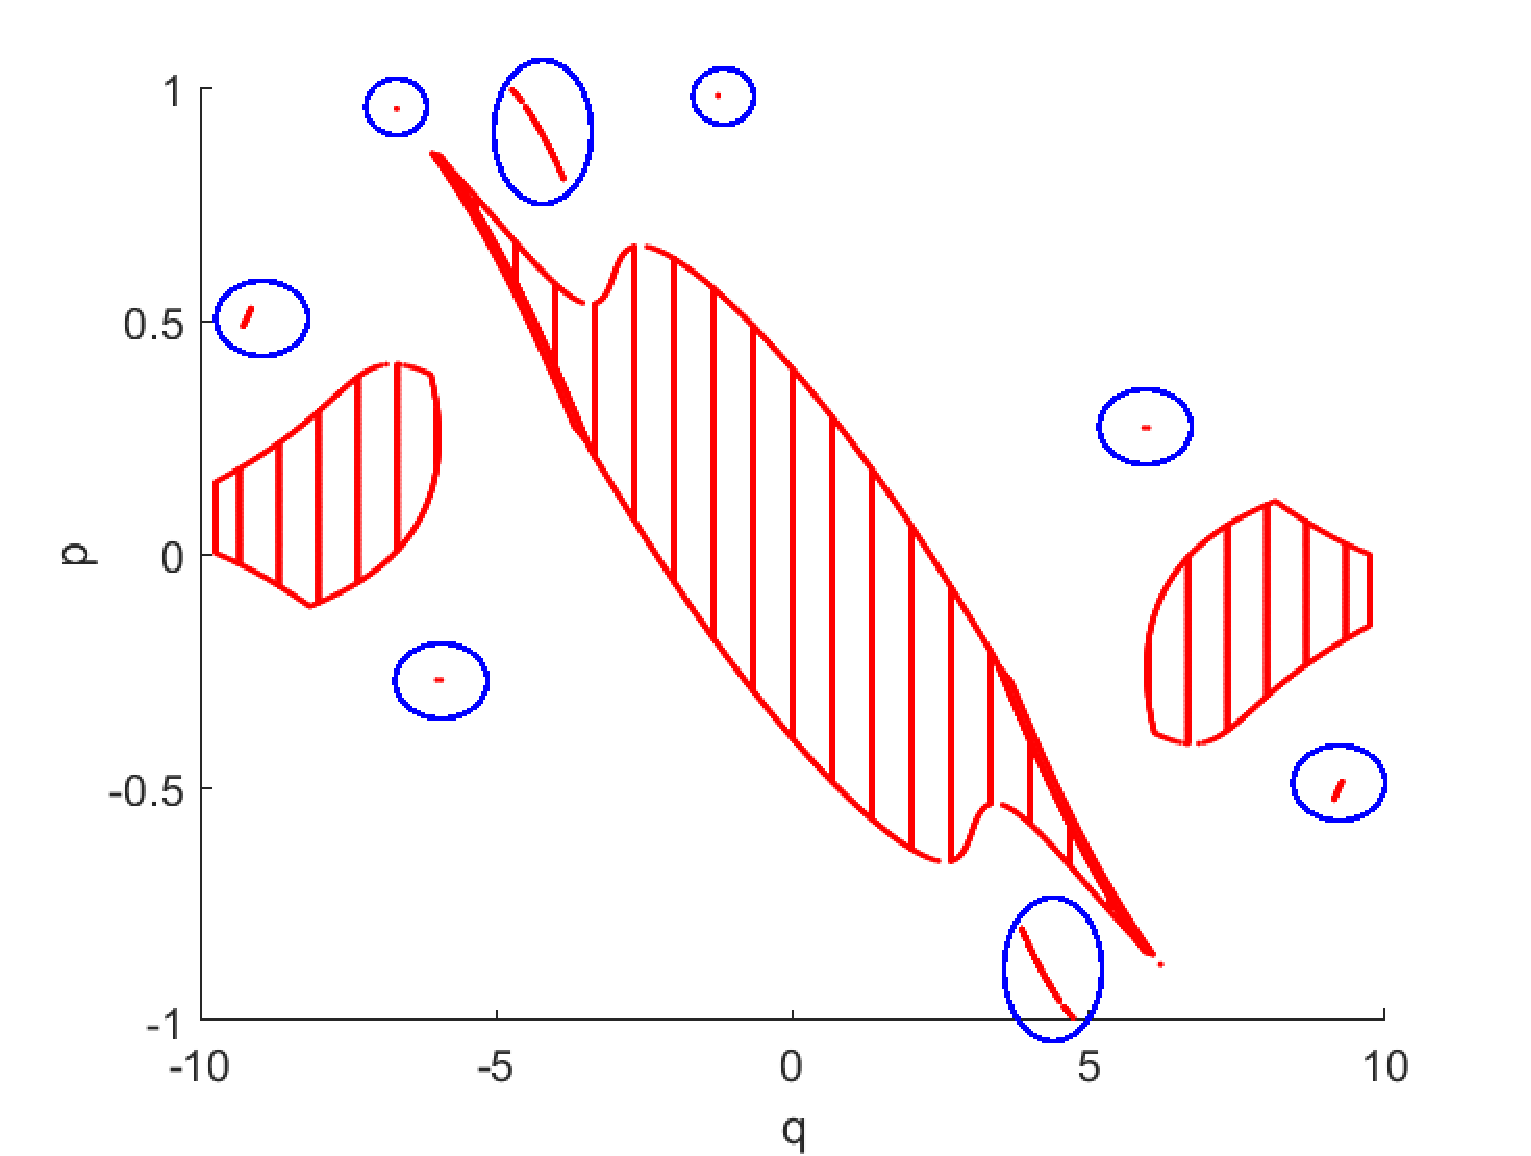
\includegraphics[width=0.7\textwidth]{boundaries_ray_mapping_tir}
  \end{center}
  \caption{\textbf{Rays distribution at target PS of the TIR-collimator.}
 The $\variabile{q}$-axis is divided into $\textrm{Ni}=30$ bins, the $\variabile{p}$-axis is divided into $\nbin = 100$ bins. Using the ray mapping method only few rays are traced from the target to the source (red dots). Because of numerical error, few rays outside the region with positive luminance are found (Rays rimmed in red).}
\label{fig:boundaries_TIR_ray_mapping}
 \end{figure}
The inverse ray mapping detects $9$ different paths from the source to the target. 
We observe that $5$ of them are paths that we expected from PS ray tracing (see Chapter \ref{chap:boundaries_alpha}). 
The inverse ray mapping also detect the following paths:
\begin{equation}
\begin{array}{llll}
\Pi_6&=(1,2,9,8,7,12), & \Pi_7&=(1,2,5,6,7,12), \\
\Pi_8&=(1,2,2,7,12),& \Pi_9&=(1,7,12),\\
\Pi_{10}&=(1,2,4,6,7,12),& \Pi_{11}&=(1,2,10,8,7,12).
\end{array}\end{equation}
Those paths are due to numerical error. Indeed, the bisection method and the inverse ray tracing depend a given tolerance. We remark that in the inverse ray tracing, the intersection between the ray and the lens (line $2$) is computed using the Newton-Raphson procedure which leads to numerical error as well.
In order to detect only the boundaries of the regions formed by the rays that follow the \textit{physical} $\Pi_{\variabile{j}}$ with $\variabile{j}\in\{1, \cdots, 5\}$, we check the index of refraction that every ray has once it arrives at the source.
If this is equal to the same index of \point{S} ($\n=1$ for the TIR-collimator), then the ray follows a physical path, otherwise it is discarded and it is not considered for the intensity calculation. This gives the rays distribution at the target PS shown in Figure\ref{fig:boundaries_TIR_ray_mapping1}. We observe that $5$ different paths are found. These are the same paths we obtained using PS ray tracing (see Chapter \ref{chap:boundaries_alpha}).
\begin{figure}[h]
  \begin{center}
  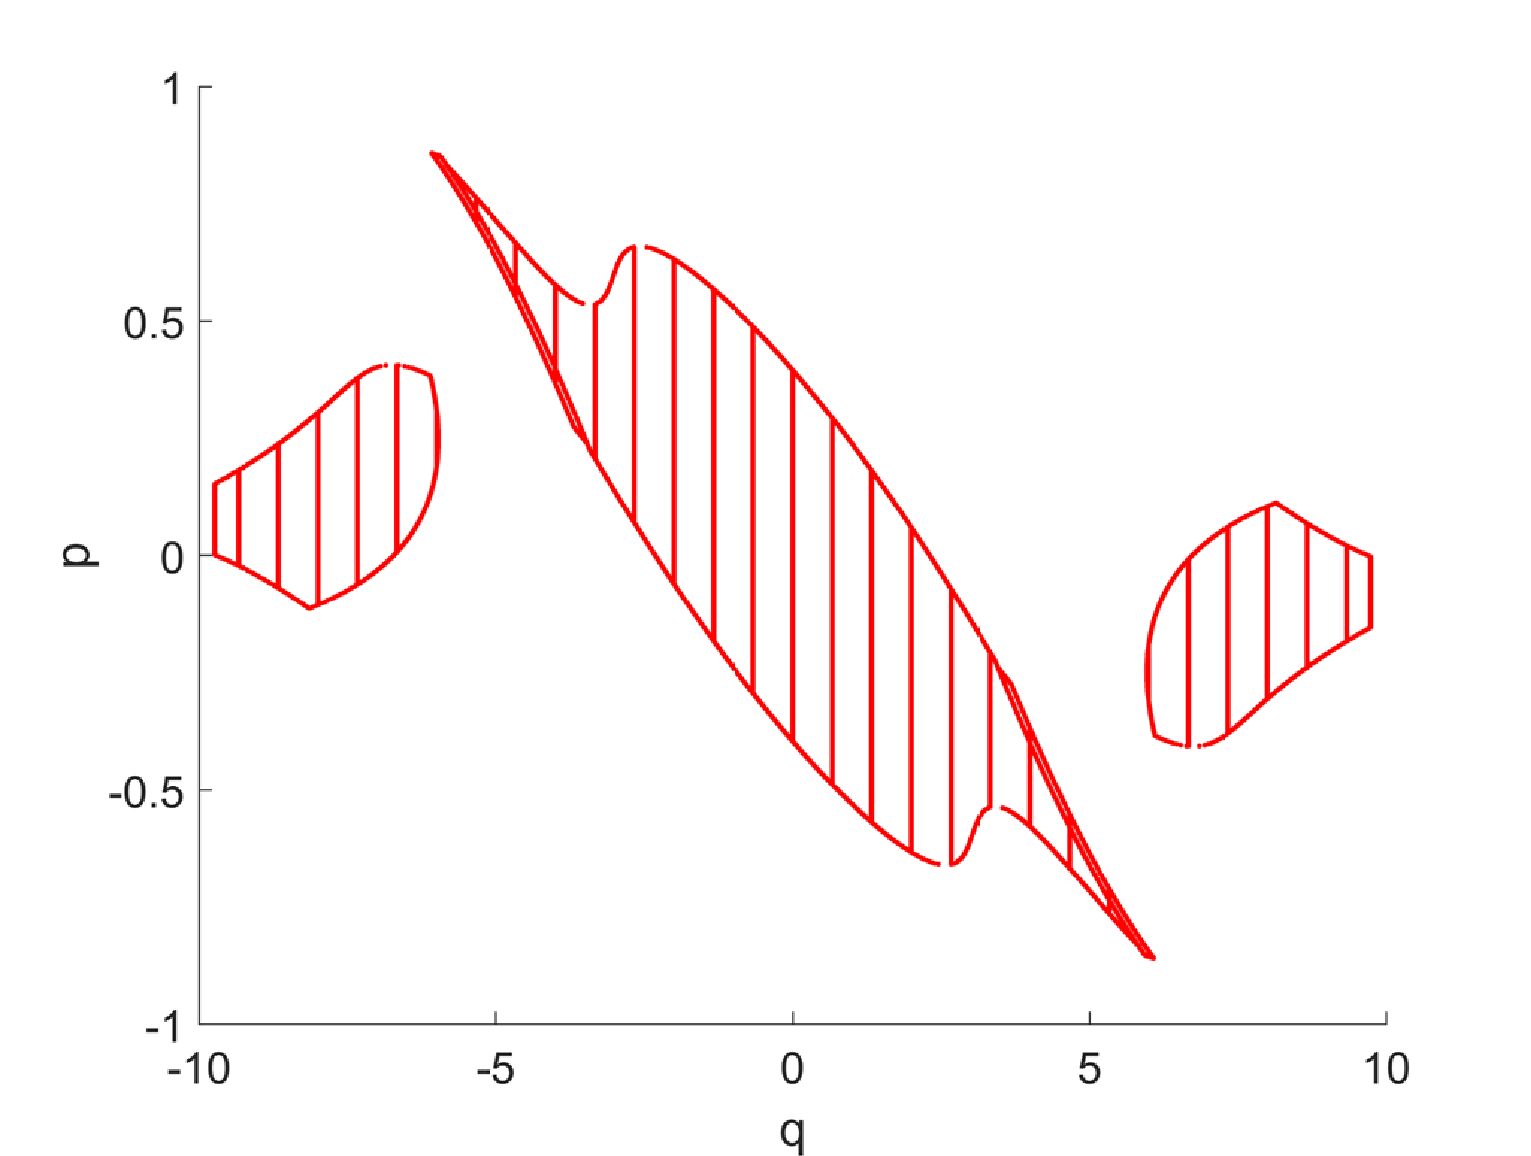
\includegraphics[width=0.7\textwidth]{boundaries_ray_mapping_tir2}
  \end{center}
  \caption{\textbf{Rays distribution at target PS of the TIR-collimator.}
 The $\variabile{q}$-axis is divided into $\textrm{Ni}=30$ bins, the $\variabile{p}$-axis is divided into $\nbin = 100$ bins. Considering only the rays that arrive to the source with the correct index of refraction ($\nline=1$), the regions with positive luminance are computed correctly.}
\label{fig:boundaries_TIR_ray_mapping1}
 \end{figure}
Figure \ref{fig:boundaries_TIR_ray_mapping1} shows that the rays on the boundaries $\partial$\set{R}{}{}$(\Pi_{\variabile{j}})$ are determined for every path $\Pi_{\variabile{j}}$ with $\variabile{j}\in\{1, \cdots, 5\}$. Moreover, some rays inside the boundaries are traced. This is related to the fact that we divide the target PS along the $\variabile{q}$-axis into $\textrm{Ni}=30$ bins. As a consequence, all the rays located at the end points of every bin are traced. \\
\indent The target PS intensity $\hat{I}_{\textrm{PS}}$ is calculated using Equation \ref{}. The profile of $\hat{I}_{\textrm{PS}}$ obtained form inverse ray mapping with $\textrm{Ni}=30$ is depicted in Figure \ref{fig:intensity_tir_raymapping} with the red line. It is compared with the reference intensity (blue line) that is given by QMC ray tracing with $10^7$ rays. The picture shows that the inverse ray mapping method calculates the intensity correctly.
\begin{figure}[t]
  \begin{center}
  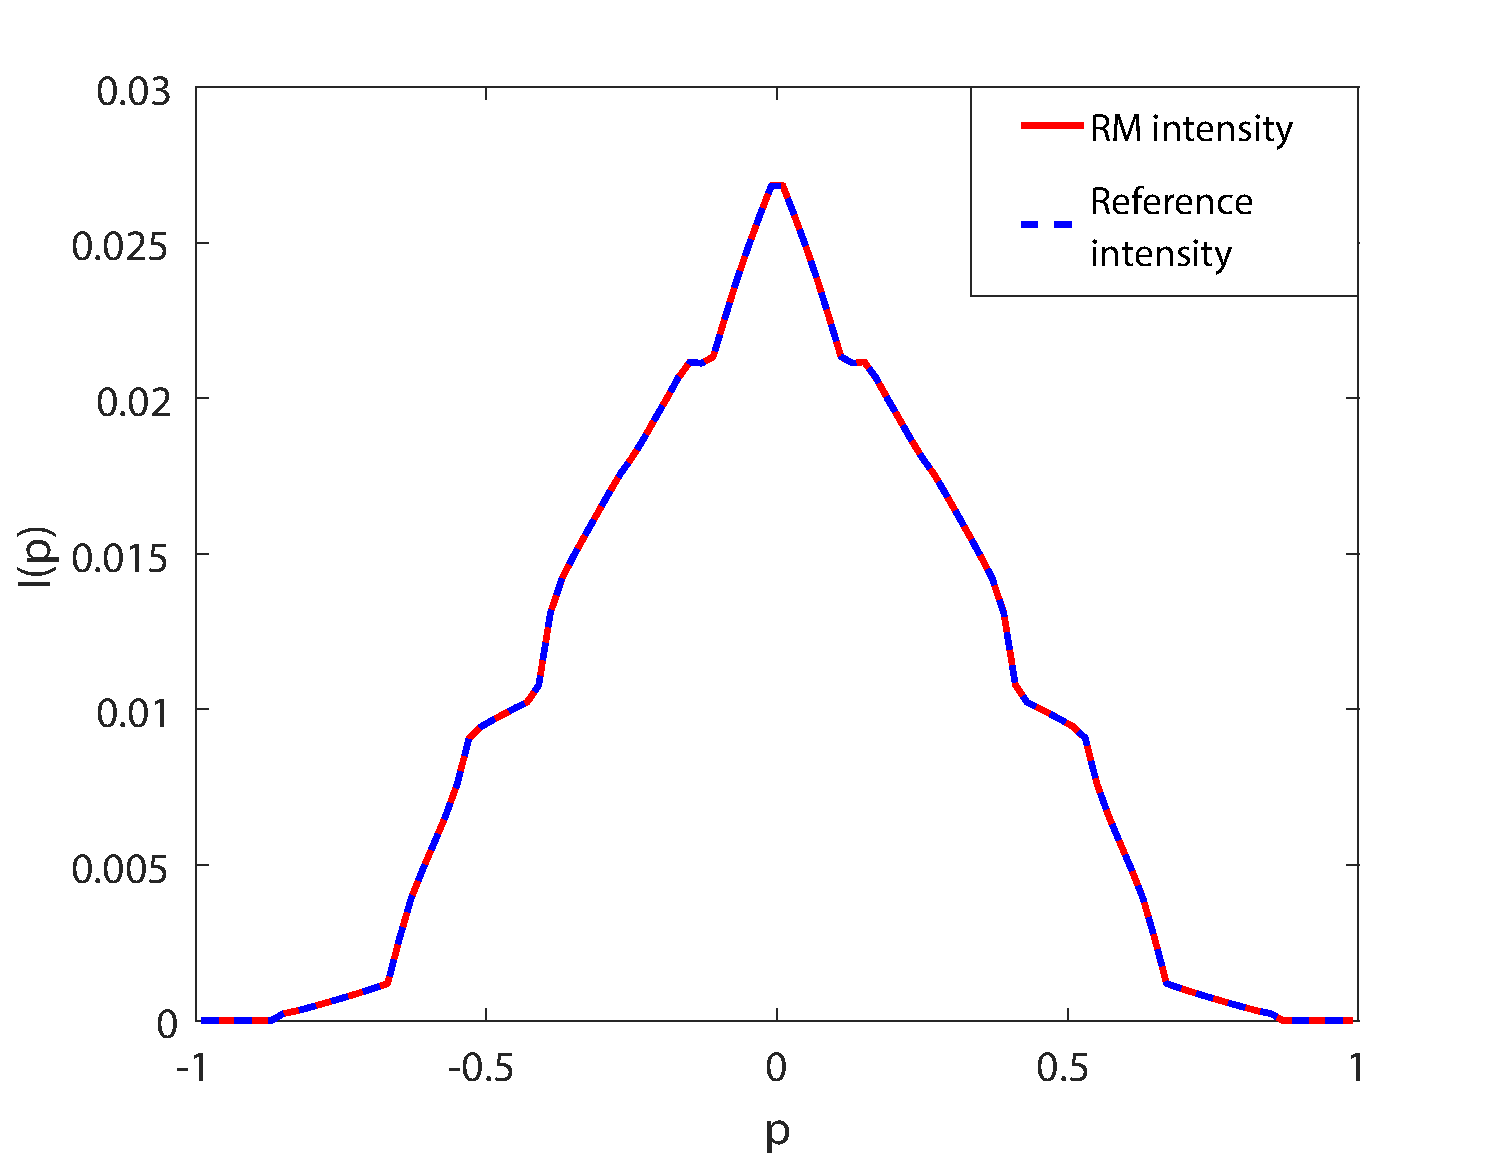
\includegraphics[width=0.7\textwidth]{intensity_tir_raymapping}
  \end{center}
  \caption{\textbf{Profile of the intensity for the TIR-collimator.}
 The ray mapping intensity is calculated dividing the $\variabile{q}$-axis into $\textit{Ni}=30$ bins. The reference intensity is obtained from QMC ray tracing with $10^7$ rays.}
\label{fig:intensity_tir_raymapping}
 \end{figure}
\\ \indent 
Finally, we compare the inverse ray mapping with QMC ray tracing. The errors plot in a logarithmic scale is shown in Figure \ref{fig:error_tir_raymapping}.
\begin{figure}[t]
  \begin{center}
  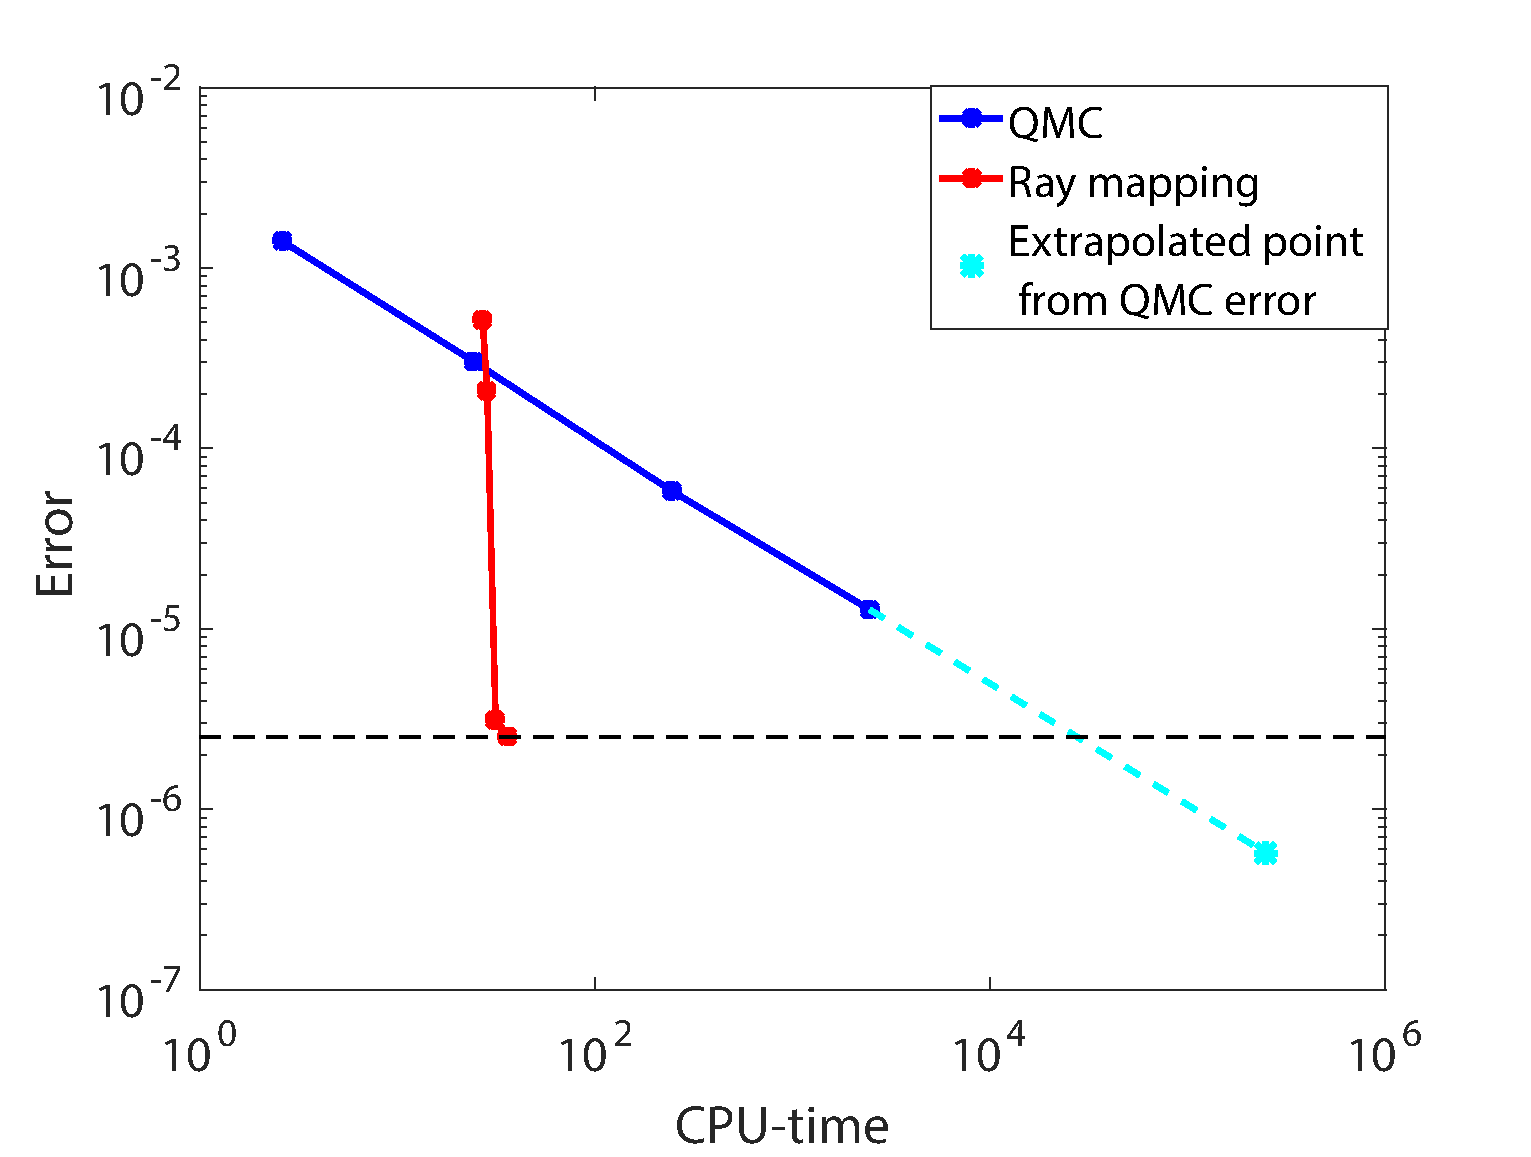
\includegraphics[width=0.7\textwidth]{error_tir_raymapping}
  \end{center}
  \caption{\textbf{Profile of the intensity for the TIR-collimator.}
 The ray mapping intensity is calculated dividing the $\variabile{q}$-axis into $\textrm{Ni}=30$ bins. The reference intensity is obtained from QMC ray tracing with $10^7$ rays.}
\label{fig:error_tir_raymapping}
 \end{figure}
% Error
\section{Results for a parabolic reflector}\label{sec:PR}
%The parabolic reflector shown in Fig. \ref{fig:parabolic_reflector} is a very challenging example of optical system. Indeed, the rays that propagate through such a system can reflect many times along the left and the right mirror 
%% Difference between PR and cup (show tree), no analytic boundaries
%% Bisection procedure
%% Divide into bins
%% Stopping criterion
%% Intensity
%% Error
